168. \begin{figure}[ht!]
\center{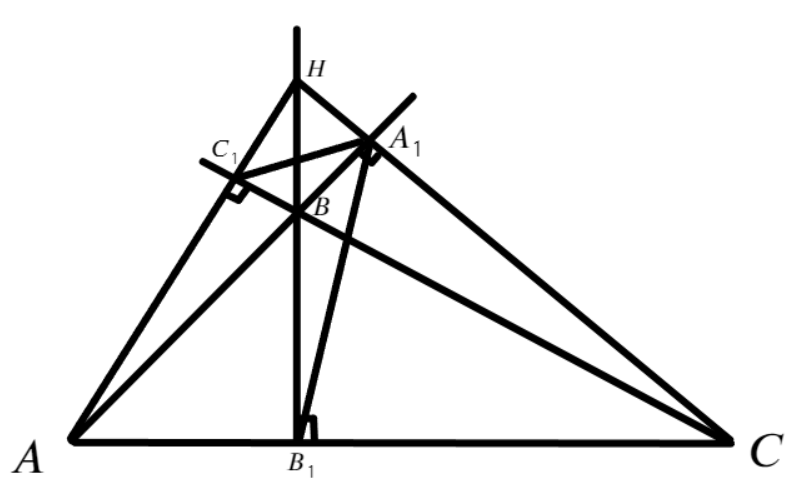
\includegraphics[scale=0.35]{g9-168.png}}
\end{figure}\\
а) Найдём $\angle A_1BC=180^\circ-120^\circ=60^\circ,\ \angle A_1CB=90^\circ-60^\circ=30^\circ,$ тогда $\angle ACH=20^\circ+30^\circ=50^\circ.$\\
б) В четырёхугольнике $AC_1A_1C$ угол, образованный стороной $AC_1$ и диагональю $CC_1,$ равен углу, образованному противоположной стороной $CA_1$ и другой диагональю $AA_1,$ значит он является вписанным и поэтому $\angle C_1A_1A=\angle C_1CA=20^\circ.$ Тогда $\angle HA_1C_1=90^\circ-20^\circ=70^\circ.$\\
в) В четырёхугольнике $B_1BA_1C$ угол, сумма противоположных углов $B_1$ и $A_1$ равна $90^\circ+90^\circ=180^\circ,$ значит он является вписанным и поэтому
$\angle A_1B_1B=\angle A_1CB=30^\circ.$\\
